\chapter{Minecraft as a Simulation Environment for MicroPsi 2}
The objective of this project is to build and test an interface in between MicroPsi and Minecraft, so that a Minecraft world can be used as a simulation environment for experiments within the MicroPsi framework, which will act as an artificial player. To make the new simulation environment monitorable, a visualisation of the Minecraft world has been implemented into the web interface. The following section gives an overview of the implemented modules.

\section{Overview}
The modular architecture of MicroPsi allows it to add new simulation environments (or worlds, as they are called in MicroPsi) fairly easily. To communicate with a MicroPsi node net, a world needs an interface, which is called \emph{world adapter}. The \emph{world adapter} has to define \emph{data sources} and \emph{targets}. It fills the sources with data from the world and writes the targets to the world. The node net does the opposite: it reads from the sources and writes into the targets. This enables a feedback loop in between the world and the node net. Furthermore, the \emph{world adapter} provides a step function, that advances the world and is called by the MicroPsi world runner frequently.

Looking at the Minecraft side, communication with a Minecraft Server typically requires a constant flow of data packets going in and out. Most third party clients, including Bots, facilitate their own event loops. To add a Minecraft world to MicroPsi, the demands of both sides have to be met.

The contributions of this project are divided into the three modules \texttt{minecraftWorldadapter}, \texttt{minecraftClient} and \texttt{minecraftVisualisation}. The resulting architecture is displayed in figure~\ref{uml_mc}. The \texttt{minecraftClient} manages the communication with the Minecraft server, provides convenient functions and data structures for sending and responding to packets and stores and constantly updates a simple representation of the environment data it receives from the server. The \texttt{minecraftVisualisation} module generates 3D-Images that display the current state of the Minecraft environment, based on the data it receives from the \texttt{minecraftClient}. What ties it all together is the \texttt{minecraftWorldadapter}. It provides a step function that advances both the \texttt{minecraftClient} and the \texttt{minecraftVisualisation} and is called itself by the world runner of the MicroPsi framework. Furthermore it defines and updates the \emph{data sources} and \emph{targets}.

\begin{figure}[h]
  \centering
    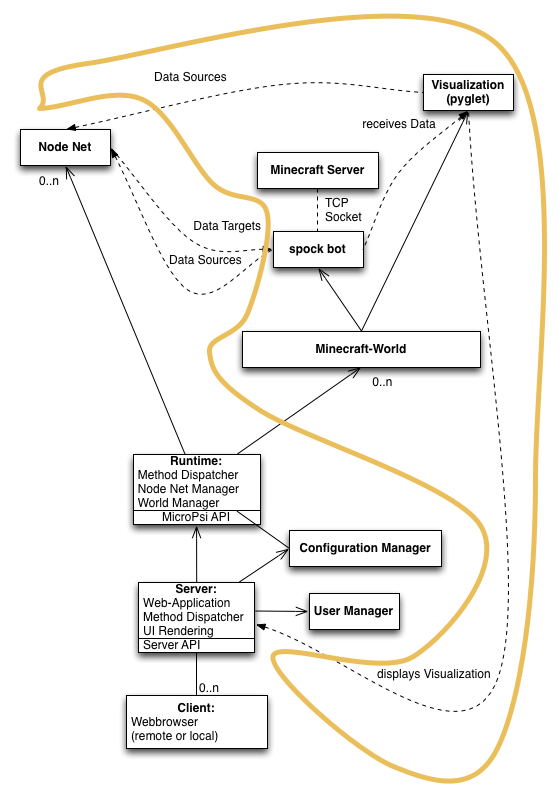
\includegraphics[width=10cm]{graphics/UML_MicroPsi_mit_spock_und_rahmen}
  \caption{The new architecture of MicroPsi with the Minecraft interface. New modules are framed orange.}
  \label{uml_mc}
\end{figure}

The \texttt{minecraftVisualisation} module can be exchanged or cut off completely very easily, as no other modules depend on it. Instead of the visualisation, a placeholder image can be displayed in the webinterface, which does not effect the functionality of simulation. The \texttt{minecraftVisualisation} module itself depends on the data structures of the \texttt{minecraftClient} though. This means, exchanging the \texttt{minecraftClient} would require adjustments of the \texttt{minecraftVisualisation}, to still function as intended. The same holds for the \emph{data sources} and \emph{targets} in the \texttt{minecraftWorldadapter}.

    \section{Using \texttt{Spock} as the \texttt{minecraftClient}}

As mentioned before, the purpose of the \texttt{minecraftClient} is to manage the communication with the Minecraft Server and to provide a representation of the agent's environment.

The calculation of the simulation environment, does not take place in MicroPsi itself, but on a regular Minecraft Server. Instead, \texttt{Spock} is integrated into MicroPsi and represents the simulation world towards it. \texttt{Spock} communicates with the Minecraft server via the Client-Server-Protocol and provides data that can be used as \emph{data sources} for the world adapter and translates the data from the \emph{data targets} to actions in the simulation environment. That way, to MicroPsi it looks like \texttt{Spock} is the simulation environment itself, where in fact it's the interface to the game world server.

The original event loop of the bot framework had to be dissolved and rebuilt as a \texttt{advanceClient} function that is called as a part of the world adapter's step function. The event-loop and -handling of Spock had to be slightly modified to work with MicroPsi. It should be noted, that the frequency, with which the framework steps the bot, has to be at least chosen high enough, so that Spock is able to send the necessary keep-alive-signals, to not get kicked from the server.

For every iteration of the event loop, the \texttt{minecraftClient} reads incoming data from the socket, dispatches the read packages appropriately and eventually checks the MicroPsi \emph{data targets} to perform an action --- if necessary~(see figure~\ref{spock_loop}). Note, that the described event loop of the original \texttt{Spock} is not a loop anymore but each iteration is invoked as a part of the world adapters step function.


\begin{wrapfigure}{r}{0.3\textwidth}
  \begin{center}
    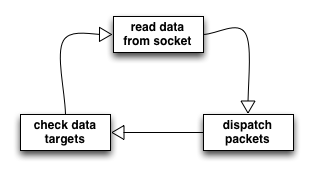
\includegraphics[width=0.3\textwidth]{graphics/spock_eventloop}
  \end{center}
  \caption{The \texttt{minecraftClient}'s event loop}
  \label{spock_loop}
\end{wrapfigure}

Eventually, useful data sources had to be picked and a system of data targets and their translation to actions had to be implemented. In most cases, performing actions means to let spock send a specific set of packets to the Minecraft server.

        \subsection{Overview of the minecraftClient}
The \texttt{minecraftClient} is heavily based on Spock, the Minecraft bot framework developed by Nick Gamberini as an educational project. It consists of several classes. The main class, \texttt{minecraftClient}, holds references to instances of the classes BoundBuffer,  World and Packet. Furthermore basic data structures are stored as cflags, mcdata.

The class BoundBuffer is an implementation of a buffer that matches the particular needs of sending and receiving Minecraft packets.

The class World holds the internal representation of the gameworld. It brings functions and datastructures/classes itself to represent chunks and to obtain information about which block sits where.

The class Packet represents a Minecraft packet and brings functions to encode and decode a packet (read from a BoundBuffer) to get to it's payload or to be able to send it to the Server.

The file packet handlers.py provides a class for each packet that the client is supposed to deal with by default. The following listing gives an example. %TODO why does not _ Latex compile


		\begin{figure}[ht]
			\centering
			\begin{minipage}{11cm}
				\begin{pseudocode}
#Chunk Data - Update client World state
@phandle(0x33)
class handle33(BaseHandle):
	@classmethod
	def ToClient(self, client, packet):
		client.world.unpack_column(packet)
					\end{pseudocode}
				\caption{Handling a Chunk Data packet}
				\label{packet_handling}
			\end{minipage}
		\end{figure}

The dictionary cflags provides the Socket codes.
The file mcdata.py provides dictionaries for the datatypes, blocktype codes, packet names and structures of packets of the Minecraft protocol.

In the file nbt.py several classes for dealing with the NBT file format exist.

The file timer.py contains the classes EventTimer, TickTimer and ThreadedTimer which provide Timing.

The client sets up a socket to the server, starts of with a handshake and then facilitates packet based communication with the server.

        \subsection{Extensions to the \texttt{minecraftClient}}
It was aimed for to extend the original client in a way. That it would fit in nicely as a simulation world for MicroPsi.
        
A reference to the new class PsiDispatcher has been added to the \texttt{minecraftClient}. It's purpose is to check the World adapters data targets frequently and invoke appropriate actions, if necessary. The following figure gives a simplified view of the resulting architecture.

The event loop has been replaced by the function \texttt{advanceClient} that is called for every simulation step. For example, one iteration could mean receiving and storing new block data from the Minecraft Server, sending default responses to the received packets, checking the MicroPsi data targets for moving and if necessary send a "Player Position" packet to the Minecraft server.

\begin{figure}[h]
  \centering
    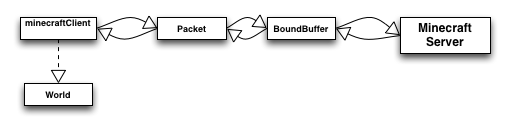
\includegraphics[width=10cm]{graphics/spock_overview}
  \caption{An overview of the most import classes of the \texttt{minecraftClient} in respect to the communication with a Minecraft Server}
  \label{spock_overview}
\end{figure}

    \section{Module \texttt{minecraftVisualisation}}
That being said, the other important part of this project is the visualisation component. It contains classes that provide an interface to the OpenGL context that is the visualisation. This sections gives an overview about what datasources the visualisation uses and how it could be replaced or extended. Inside the world adapter's step function, the visualisation module is called to generate a 3D model of the Minecraft world and the agent within. There are two main reasons for this. The first reason is, that the agent's behaviour within the simulation environment is supposed to be visually monitored from the MicroPsi web interface --- in a both effective and pleasurable manor. The second reason is, that the image data is supposed to be processed by the node net as a data source itself in the future.

The module \texttt{minecraftVisualisation} consists of two classes. The class \texttt{Window} inherits from pyglet.window.Window and therefore initialises the OpenGL context. For every call of the advanceVisualisation function it updates the 3D model according to world representation inside the minecraftClient and is rendered. A .png snapshot of the framebuffer is generated and displayed in the web interface.

The class Model is also called as a part of the advanceVisualisation function. It contains functions for adding and removing blocks from the OpenGL canvas. The textures for the blocks are loaded from PNG images and stored as pyglet.graphics.TextureGroup and assigned to vertices when needed.

The visualisation component reads from Spock's internal gameworld representation to generate the 3D model. This means, that from pure Minecraft world data a 3D-visualisation has to be generated from within the MicroPsi Python Code. It should contain a perspective that gives a good overview over the bots environment to forward to the web interface, as well as a the agent's first person perspective, to function as a data source in the future.  

The visualisation is in it's core based on ``Minecraft'' by Michael Fogleman.

\begin{figure}[h]
  \centering
    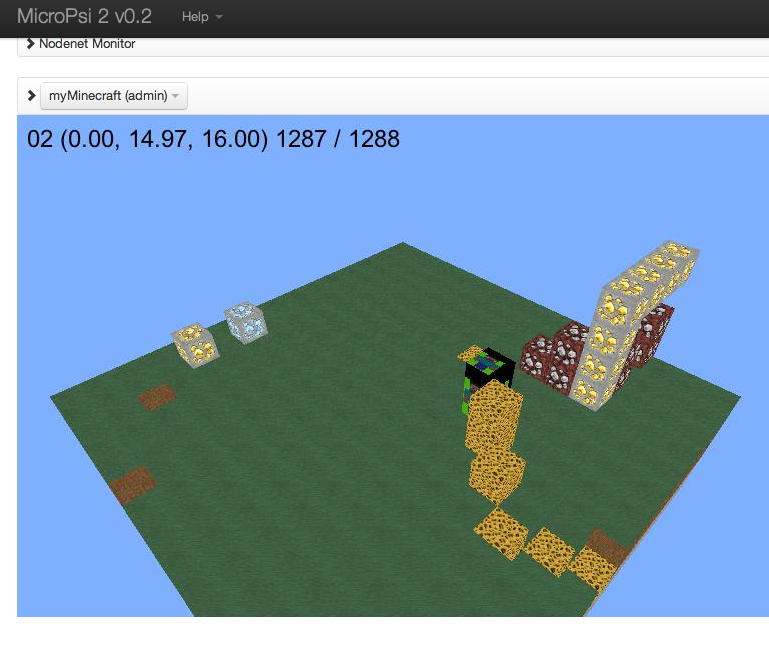
\includegraphics[width=10cm]{graphics/visualisation_screen}
  \caption{An Image generated by the visualisation component}
  \label{vis_screen}
\end{figure}

Specifically, the representation of the chunk, the agent is located in, is fetched and for each solid cube in this chunk, a corresponding cube is rendered within the visualisation using Pyglet's OpenGL abstraction~(see figure~\ref{vis_screen}). Each block gets textures according to it's type. The implemented format for the textures is compatible to the widely available Minecraft texture packs. That way, the visualisation's look can be changed completely within seconds. The resulting images are exported as JPEG files. Then, they are displayed in the web interface. A refresh rate of six or more images per second creates the impression of a video stream.

Similar to spock, ``Minecraft'' by Michael Fogleman implements it's own event-loop and -handling. Again, the event loop had to be disassembled and rebuilt as a part of the world adapter's step function, which advances the visualisation with every step.

    \section{Module \texttt{minecraftWorld}}
The world adapter contains two classes. The class MinecraftWorld inherits from the MicroPsi class world and provides the the assets for the webinterface, an init function and the step function. The class Braitencraft is the name of the actual Worldadapter. In it, the \emph{data sources} and \emph{targets} are defined as dictionaries and an update function advances the life of the client.
    
\paragraph{Data Targets and sources}

As a proof of concept, datasources have been defined, that symbolize sensors that detect if a block of diamond in the current section is either before, behind, left or right of the client. The data targets are filled as a part of the world adapter update function as follows:

On the other hand, data targets have been defined for walking moving forwards, backwards, left and right.

% TODO je nach Größe des Kapitels, das hier vielleicht eine Ebene höher ziehen (versuche dich hier erstmal nur auf die fertige Lösung zu konzentrieren und warum du dich dafür entschieden hast. Es ist nicht interessant, was du sonst alles ausprobiert hast, außer dass du konkret angibst, warum du dich für die jetztige Implementierung im Vergleich zu anderen entschieden hast)

    \section{Case Study}
As a proof of concept, the Bot is placed in a chunk in which a diamond is placed. The node net has been set up, so that each diamond sensor is connected to the appropriate movement actor, as in figure\ref{nodenet_setup}.

\begin{figure}[h]
  \centering
    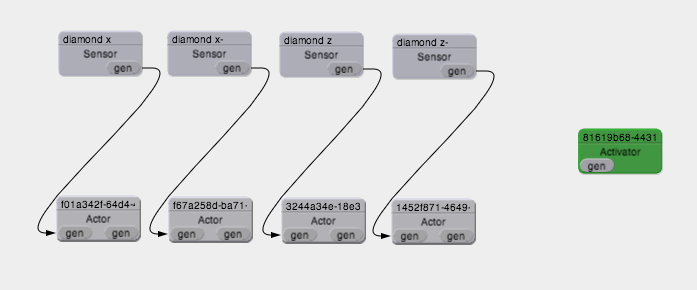
\includegraphics[width=10cm]{graphics/nodenet_setup}
  \caption{A node net setup for a Diamond-finding experiment}
  \label{nodenet_setup}
\end{figure}

If we start a simulation like this, the nodes of the sensors that point to the diamond light up green and their activation is forwarded to the actors. The bot move towards the diamond until it it closer than the threshold for the sensors to not detect the diamond anymore --- for this experiment the threshold was set to two blocks~(see figure \ref{diamond_screens})

\begin{figure}[h]
  \centering
    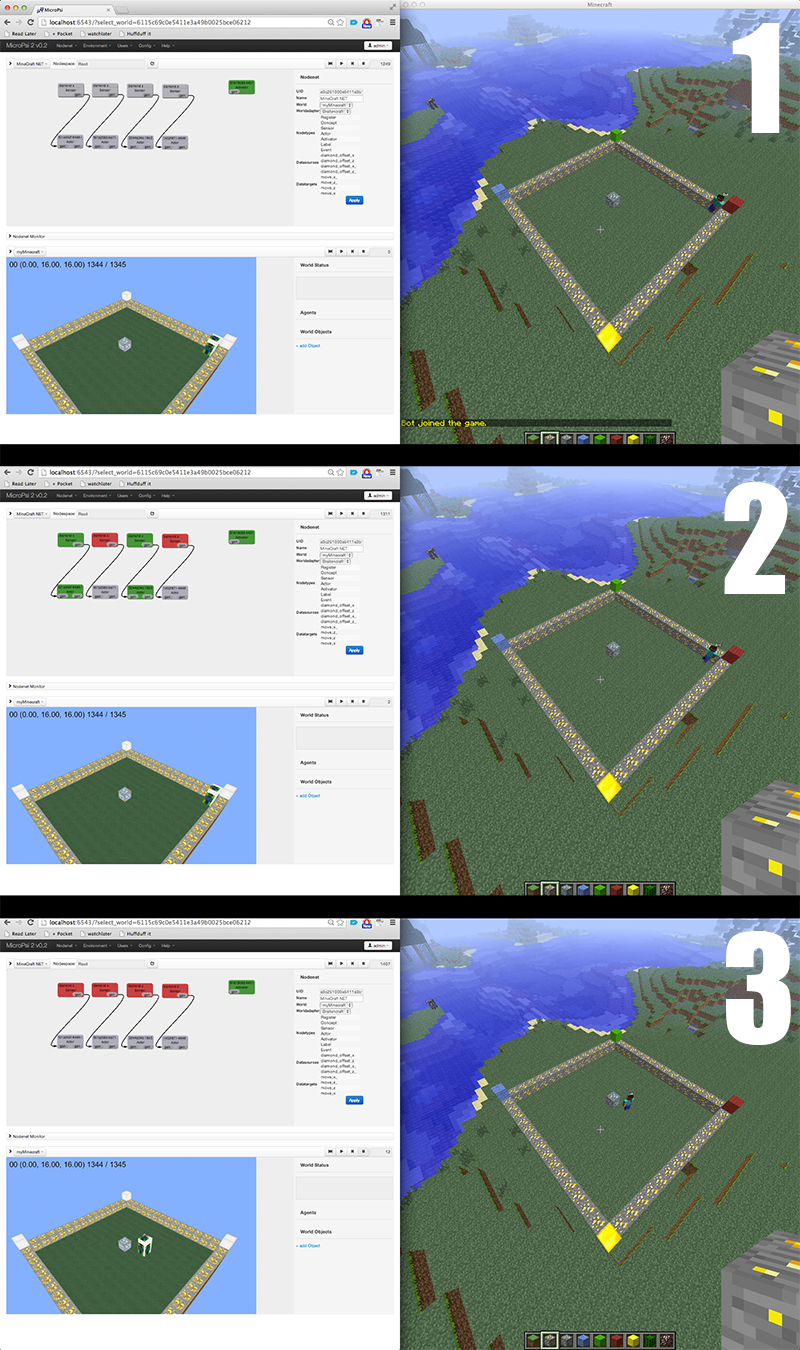
\includegraphics[width=10cm]{graphics/diamond_screens}
  \caption{Three screenshots with a Minecraft bot walking towards the diamond}
  \label{diamond_screens}
\end{figure}